\documentclass[11pt,a4paper]{article}
\usepackage[margin=22mm]{geometry}
\usepackage[T1]{fontenc}
\IfFileExists{lmodern.sty}{\usepackage{lmodern}}{}
\usepackage{tabularx,booktabs,xcolor,graphicx,longtable,float,array,enumitem}
\usepackage[hyphens]{xurl}
\usepackage{hyperref}
\hypersetup{colorlinks=true,linkcolor=blue!50!black,urlcolor=blue!50!black}
\setlength{\parindent}{0pt}\setlength{\parskip}{6pt}
\newcommand{\entry}[2]{\textbf{#1:} #2\par}
\newcommand{\todo}[1]{\textcolor{red}{\textbf{[TEAM TO FILL: #1]}}}
\renewcommand{\arraystretch}{1.15}
\setlength{\emergencystretch}{3em}\sloppy
\setlist{nosep,leftmargin=1.5em}
\begin{document}
\begin{center}\Large\textbf{23CSE455 Design Patterns}\\[4pt]\LARGE Case Study Report\end{center}

\entry{Team}{A12}
\entry{Case study}{OTT / video streaming application using React / Next.js --- \emph{Design Pattern Analysis in a Next.js-Based Video Streaming Application}}
\entry{Application}{netflx-web (Netflix clone, Next.js 13 app router, tRPC, NextAuth, Prisma, Stripe) by sadmann7. Faculty approval: approved by the course faculty for use in this case study.}
\entry{Date}{2026-10-10}
\textbf{Submission repository:} \href{https://github.com/aswathymohan-amrita/23CSE455_DP_CaseStudy}{23CSE455\_DP\_CaseStudy}, folder \texttt{A12/}\par
\textbf{Students}\par
\begin{tabularx}{\linewidth}{@{}llX@{}}\toprule
Roll number & Student name & Batch\\\midrule
AM.SC.U4CSE23161 & Swaminathan A & CSE B\\
AM.SC.U4CSE23207 & Anna Ouseph & CSE C\\
AM.SC.U4CSE23230 & Leya Paul & CSE C\\
AM.SC.U4CSE23242 & Pooja Sathyan & CSE C\\
AM.SC.U4CSE23069 & Rahul Rajan & CSE A\\\bottomrule
\end{tabularx}

\section{Application and architecture}
\entry{Original source}{\url{https://github.com/sadmann7/netflx-web}, branch \texttt{main}, no release tags; baseline commit \texttt{676e5ddd15d68fe6b83c2f9cc2494c6ece8b2258} (2024-06-12, ``Merge pull request \#11''); accessed 2026-10-10. \textbf{Licence: none} --- the repository has no LICENSE file, so all rights are reserved by the author; the code is used only for this academic analysis. Snapshot: \path{code/}.}
\entry{Environment}{TypeScript 5.0.4 on Node.js; Next.js 13.4.4 (app router + pages router for API routes), React 18.2.0, tRPC 10.28.0, NextAuth 4.22.1 with @next-auth/prisma-adapter 1.0.6 (Google OAuth), Prisma 4.14.1 on MySQL (\texttt{relationMode = "prisma"}), Stripe 12.7.0, Zustand 4.3.8, @tanstack/react-query 4.29.7, Tailwind CSS 3.3.2; catalogue data from the TMDB REST API. Analysis tools: Node.js 22.22.0, yarn 1.22.22, vitest 1.6.0, lizard 1.24.1, PlantUML + Graphviz.}
\entry{Scope}{Inspected: \path{src/server/**}, \path{src/lib/**}, \path{src/config/**}, \path{src/stores/**}, \path{src/app/**}, \path{src/components/**}, \path{src/@trpc/next-layout/**}, \path{src/env.mjs}, \path{prisma/schema.prisma}, and dependency code where a role is implemented (next-auth, prisma-adapter, zustand, tRPC, react-query). Excluded: \path{components/ui/*} (generated shadcn UI primitives), \path{styles/}, \path{public/}, \path{app/(docs)} (static help/terms text) and \path{app/api/og} (Open Graph image) --- none of them belongs to the seven case-study areas. The area-to-file map is in \path{Part1/evidence/candidates.md}.}
\entry{Architecture}{Figure~\ref{fig:arch} (source \path{Part1/diagrams/00_architecture.puml}).}
\begin{figure}[H]\centering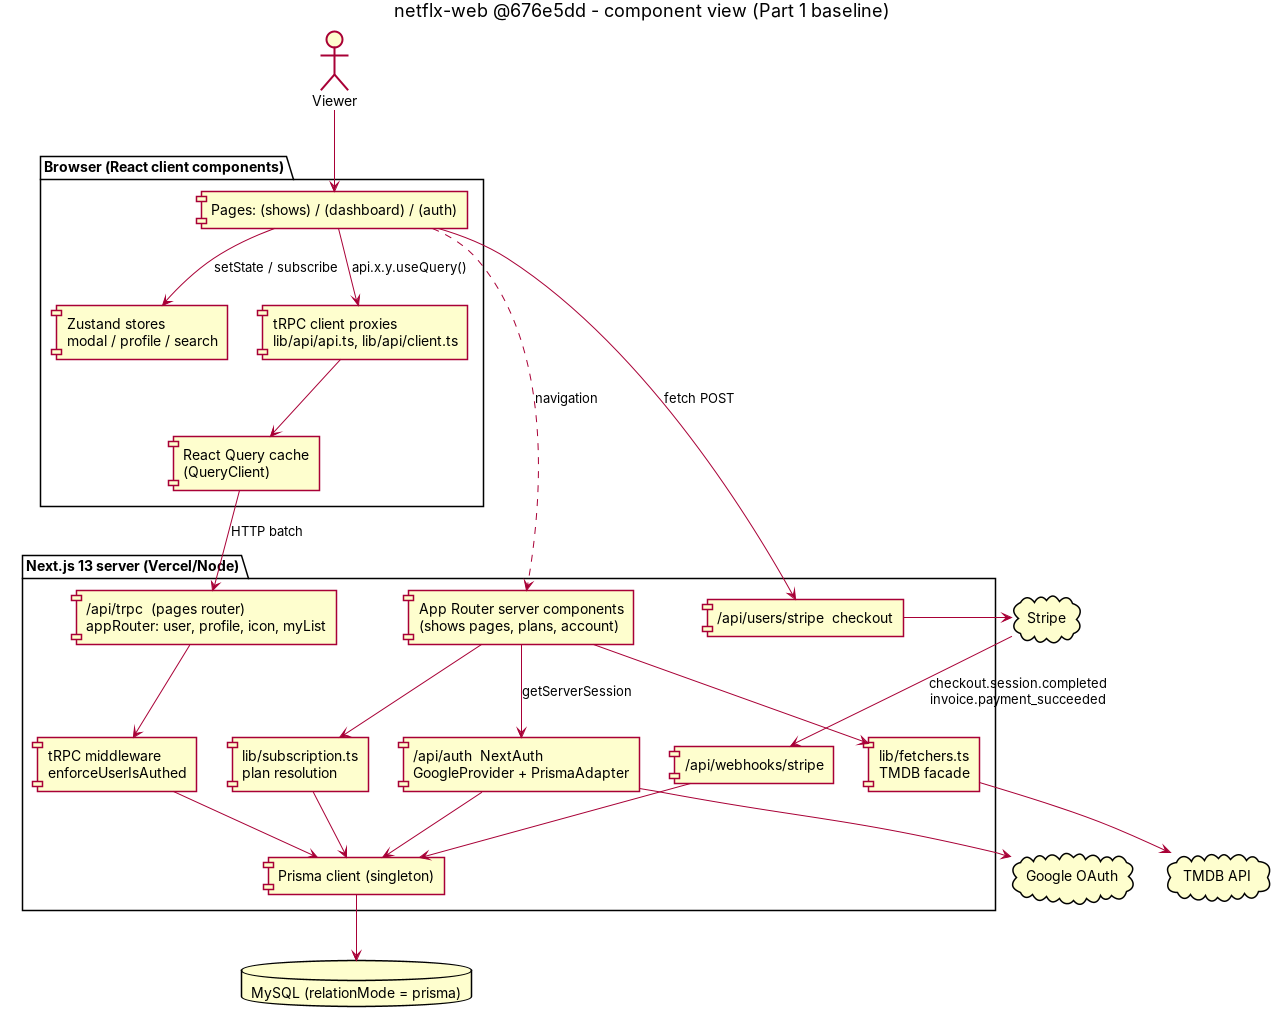
\includegraphics[width=\linewidth]{Part1/diagrams/00_architecture.png}
\caption{Component view of netflx-web at the baseline.}\label{fig:arch}\end{figure}
\textbf{Components.} \emph{Browser}: React client components (shows carousels, modal, profile screens, forms) keep UI state in three Zustand stores (modal, profile, search) and call the server through two tRPC client proxies backed by one React-Query cache. \emph{Server}: App-router server components render pages and fetch catalogue rows from TMDB through \path{lib/fetchers.ts}; the tRPC API (\path{/api/trpc}, pages router) serves user, profile, icon and My-List procedures behind an authentication middleware; NextAuth (\path{/api/auth}) signs users in with Google and stores users/sessions through the Prisma adapter; Stripe checkout (\path{/api/users/stripe}) and a Stripe webhook (\path{/api/webhooks/stripe}) maintain the subscription fields on the User row. Every server module reads configuration through the \texttt{env} proxy.

\textbf{Request flow (adding a title to My List).} A viewer clicks a poster $\rightarrow$ \texttt{ShowCard} publishes \texttt{\{show, open\}} to \texttt{useModalStore} $\rightarrow$ \texttt{ShowsContainer} renders \texttt{ShowModal}, which fetches the trailer from TMDB $\rightarrow$ ``Add to My List'' calls \texttt{api.myList.create.useMutation} on the tRPC proxy $\rightarrow$ HTTP batch to \path{/api/trpc} $\rightarrow$ \texttt{createTRPCContext} loads the session $\rightarrow$ \texttt{enforceUserIsAuthed} passes the request on $\rightarrow$ the resolver loads the profile with its list through the Prisma singleton and inserts a \texttt{MyShow} row $\rightarrow$ the modal invalidates the cached \texttt{myList.getAll} query, so the next read reloads it.
\entry{Run instructions}{\path{README.md} (team) and \path{code/README.md} (original). Setup: copy \path{.env.example} to \path{.env} (MySQL URL, Google OAuth, TMDB key, Stripe keys), \texttt{yarn install} (runs \texttt{prisma generate}), \texttt{npx prisma db push}, \texttt{yarn dev}, \texttt{yarn stripe:listen}. \textbf{Actual result in the analysis environment:} \texttt{npx tsc --noEmit} passes on the baseline (\path{test_result/baseline/typecheck.log}); \texttt{next build} stops at \texttt{next/font} because the sandbox cannot download Inter from Google Fonts (\path{test_result/baseline/build.log}) --- an environment limit, not a code error; the baseline repository contains no tests. Prisma engines could not be downloaded either, so the database was replaced by an in-memory fake in all tests.}

\section{Part 1 Pattern discovery}
\entry{Method}{(1) Listed the entry files of each of the seven areas and read them completely. (2) Followed every import/call one hop, including into \path{node_modules} when a role is played by a dependency (versions pinned by \path{yarn.lock}). (3) For each candidate, recorded intent, the role relationships and the delegation that happens at run time; a candidate was confirmed only when all three are visible in code, never from a name, comment or LLM statement alone. (4) Line ranges were checked by script: \path{Part1/evidence/verify_locations.py} (all cited ranges exist and start at the named symbol: 90/90, \path{Part1/evidence/location_check.log}) and an independent bracket-matching locator (\path{Part2/evidence/locate.py}) for end lines, which found and fixed two wrong end lines. (5) Rejected and uncertain candidates were recorded with reasons. The first pass was done with an LLM (section 5) and every claim was then checked against the source.}
\subsection{Totals at the baseline}
\entry{Confirmed pattern types}{Chain of Responsibility, Singleton, Observer, Decorator, Adapter, Strategy, Facade, Composite, Proxy, Read-Through Cache --- \textbf{10}}
\entry{Confirmed pattern instances}{\textbf{15} independent collaborations (table below).}
\entry{Concrete participant classes}{\textbf{33} implementations of variable roles (ConcreteHandler, ConcreteObserver, ConcreteStrategy, ConcreteComponent/Decorator, Adapter, Singleton, Facade module, Composite routers, Proxy, Cache). Many are React function components or modules, not classes; we do not invent classes for them.}
\entry{Unique participant symbols}{\textbf{55} distinct mapped symbols in the repository (e.g.\ \texttt{ShowsContainer}, \texttt{prisma}, \texttt{AppRouter} counted once although they take part in several instances) plus \textbf{12} dependency symbols (e.g.\ \texttt{PrismaAdapter}, zustand \texttt{persist}); list in \path{Part1/evidence/part1_patterns.py}.}
\entry{Rejected and uncertain candidates}{\textbf{6 rejected}, \textbf{4 uncertain} (section 2.4). Observation scope: static reading of the baseline source plus type checking; no run with real Stripe, TMDB or Google credentials.}
\subsection{Pattern inventory}
\begin{longtable}{@{}p{3.3cm}p{8.3cm}cc@{}}\toprule
Pattern type & Instance names & Instances & Concrete\\\midrule\endhead
Chain of Responsibility & Authenticated Procedure Pipeline & 1 & 1\\
Singleton & Shared Prisma Database Client; Stripe API Client & 2 & 2\\
Observer & Show Modal Selection; Active Profile Selection; Search Results Broadcast & 3 & 15\\
Decorator & Persisted Profile Store & 1 & 3\\
Adapter & NextAuth Prisma Persistence Adapter & 1 & 1\\
Strategy & Sign-in Provider Strategy & 1 & 1\\
Facade & TMDB Catalogue Facade & 1 & 1\\
Composite & API Router Tree & 1 & 5\\
Proxy & Pages-Router tRPC Client Proxy; App-Router tRPC Client Proxy; Environment Secret Guard & 3 & 3\\
Read-Through Cache & My List Query Cache & 1 & 1\\
\midrule Total & & 15 & 33\\\bottomrule\end{longtable}
\textbf{Mapping to the seven areas.} User management: Active Profile Selection, Persisted Profile Store, API Router Tree. Video catalogue: TMDB Catalogue Facade, Show Modal Selection, Search Results Broadcast. Subscription: Stripe API Client (plans resolved in \path{lib/subscription.ts}). Authentication: Authenticated Procedure Pipeline, Sign-in Provider Strategy, NextAuth Prisma Persistence Adapter, Shared Prisma Database Client. Content access: Authenticated Procedure Pipeline (server), Environment Secret Guard (configuration secrets); the profile PIN gate is only an uncertain candidate. Caching: My List Query Cache, (rejected) server caching proxy. Recommendation: \textbf{no pattern} --- the home page shows fixed TMDB lists (trending, top rated, five genre ids); no user signal is used.
\subsection{One record for each pattern instance}
\subsubsection*{Authenticated Procedure Pipeline}
\entry{Pattern type and category}{Chain of Responsibility --- Behavioral (GoF); tRPC middleware idiom}
\entry{Purpose and origin}{Problem: every private procedure must reject anonymous callers. Origin: application (create-t3-app scaffold) on framework.}
\textbf{Participant mapping}\par
\begin{tabularx}{\linewidth}{@{}p{3.4cm}X>{\raggedright\arraybackslash}p{6.0cm}@{}}\toprule Pattern role & Actual class, interface and function & File and line range\\\midrule
Handler & tRPC MiddlewareFunction created by t.middleware & dependency @trpc/server@10.28.0\\
ConcreteHandler & enforceUserIsAuthed & \path{code/src/server/api/trpc.ts:109-119}\\
Chain assembly & protectedProcedure = t.procedure.use(enforceUserIsAuthed) & \path{code/src/server/api/trpc.ts:129}\\
Terminal handler & procedure resolvers e.g. profileRouter.getAll & \path{code/src/server/api/routers/profile.ts:7-15}\\
Client & createNextApiHandler (tRPC HTTP entry point) & \path{code/src/pages/api/trpc/[trpc].ts:8-19}\\
\bottomrule\end{tabularx}
\entry{Evidence}{Problem: every private procedure must reject anonymous callers. enforceUserIsAuthed inspects ctx.session and either throws TRPCError UNAUTHORIZED (stops the chain) or calls next(\{ctx\}) with a narrowed session, passing the request to the next link. protectedProcedure attaches the handler once; 18 of 19 procedures in user/profile/icon/myList routers are built on it, so the check runs before each resolver without being repeated.}
\entry{Diagram}{\path{Part1/diagrams/01_cor_authenticated_procedure_pipeline.puml} (editable), \path{Part1/diagrams/01_cor_authenticated_procedure_pipeline.png}}
\begin{figure}[H]\centering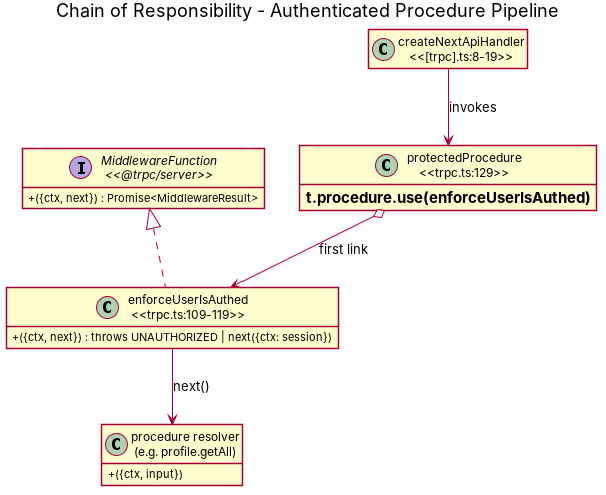
\includegraphics[width=0.62\linewidth]{Part1/diagrams/01_cor_authenticated_procedure_pipeline.png}\caption{Authenticated Procedure Pipeline}\end{figure}
\entry{Verification}{Confirmed. Characterization tests: anonymous caller -> UNAUTHORIZED, signed-in caller reaches the resolver with its id, public procedure stays open (\path{tests/characterization.test.ts}). Alternative considered: Decorator (procedure.use wraps) --- rejected because each middleware decides whether to pass the request on, which is the defining CoR property. Reviewer: \todo{roll no./name}}
\subsubsection*{Shared Prisma Database Client}
\entry{Pattern type and category}{Singleton --- Creational (GoF)}
\entry{Purpose and origin}{Problem: Next.js hot reload re-evaluates modules, which would open a new connection pool each time. Origin: application (create-t3-app scaffold).}
\textbf{Participant mapping}\par
\begin{tabularx}{\linewidth}{@{}p{3.4cm}X>{\raggedright\arraybackslash}p{6.0cm}@{}}\toprule Pattern role & Actual class, interface and function & File and line range\\\midrule
Singleton & prisma (PrismaClient instance) & \path{code/src/server/db.ts:9-14}\\
Instance holder & globalForPrisma (globalThis cache) & \path{code/src/server/db.ts:5-7,16}\\
Client & createInnerTRPCContext & \path{code/src/server/api/trpc.ts:47-52}\\
Client & authOptions.adapter = PrismaAdapter(prisma) & \path{code/src/server/auth.ts:48}\\
Client & getUserSubscriptionPlan & \path{code/src/lib/subscription.ts:6-53}\\
Client & Stripe webhook POST & \path{code/src/app/api/webhooks/stripe/route.ts:8-76}\\
\bottomrule\end{tabularx}
\entry{Evidence}{Problem: Next.js hot reload re-evaluates modules, which would open a new connection pool each time. db.ts reuses globalForPrisma.prisma if present (??) and only constructs PrismaClient once, then stores it on globalThis outside production. All server code imports the same `prisma` export.}
\entry{Diagram}{\path{Part1/diagrams/02_singleton_shared_prisma_client.puml} (editable), \path{Part1/diagrams/02_singleton_shared_prisma_client.png}}
\entry{Verification}{Confirmed by reading; behaviour reproduced in Part 3 problem 02 (9/9 cases incl. hot reload). Alternative: plain module export --- the explicit globalThis guard makes it a deliberate singleton. Reviewer: \todo{roll no./name}}
\subsubsection*{Stripe API Client}
\entry{Pattern type and category}{Singleton --- Creational (GoF); ES-module singleton idiom}
\entry{Purpose and origin}{One configured Stripe client (API key, apiVersion 2022-11-15) is created at module load and exported; the ES module cache guarantees a single instance per server process. Origin: application.}
\textbf{Participant mapping}\par
\begin{tabularx}{\linewidth}{@{}p{3.4cm}X>{\raggedright\arraybackslash}p{6.0cm}@{}}\toprule Pattern role & Actual class, interface and function & File and line range\\\midrule
Singleton & stripe (Stripe instance) & \path{code/src/lib/stripe.ts:4-7}\\
Client & Stripe webhook POST & \path{code/src/app/api/webhooks/stripe/route.ts:8-76}\\
Client & checkout/portal POST & \path{code/src/app/api/users/stripe/route.ts:14-115}\\
Client & PlansPage & \path{code/src/app/(auth)/login/plans/page.tsx:17-60}\\
Client & AccountPage & \path{code/src/app/(dashboard)/account/page.tsx:16-61}\\
\bottomrule\end{tabularx}
\entry{Evidence}{One configured Stripe client (API key, apiVersion 2022-11-15) is created at module load and exported; the ES module cache guarantees a single instance per server process. Four call sites share it instead of constructing their own. No global guard as in db.ts, so it relies on module caching only (noted as weaker form).}
\entry{Diagram}{\path{Part1/diagrams/03_singleton_stripe_client.puml} (editable), \path{Part1/diagrams/03_singleton_stripe_client.png}}
\entry{Verification}{Confirmed as module-level singleton; weaker form (no guard, relies on the ES module cache). Reviewer: \todo{roll no./name}}
\subsubsection*{Show Modal Selection}
\entry{Pattern type and category}{Observer --- Behavioral (GoF); Zustand store subscription}
\entry{Purpose and origin}{Selecting a poster calls useModalStore.setState(\{show, open, play\}) (shows-carousel.tsx:105-109). Origin: application on dependency (zustand@4.3.8).}
\textbf{Participant mapping}\par
\begin{tabularx}{\linewidth}{@{}p{3.4cm}X>{\raggedright\arraybackslash}p{6.0cm}@{}}\toprule Pattern role & Actual class, interface and function & File and line range\\\midrule
Subject & zustand StoreApi (subscribe/setState) created by create() & dependency zustand@4.3.8\\
ConcreteSubject & useModalStore & \path{code/src/stores/modal.ts:13-20}\\
Publisher (calls setState) & ShowCard onClick & \path{code/src/components/shows-carousel.tsx:93-113}\\
ConcreteObserver & ShowsContainer & \path{code/src/components/shows-container.tsx:22-65}\\
ConcreteObserver & ShowModal & \path{code/src/components/show-modal.tsx:30-296}\\
ConcreteObserver & Hero & \path{code/src/components/hero.tsx:17-102}\\
ConcreteObserver & ShowsGrid & \path{code/src/components/shows-grid.tsx:13-48}\\
\bottomrule\end{tabularx}
\entry{Evidence}{Selecting a poster calls useModalStore.setState(\{show, open, play\}) (shows-carousel.tsx:105-109). Components that called useModalStore() are subscribed by the hook and re-render when state changes: ShowsContainer/ShowsGrid open ShowModal, ShowModal fetches the trailer for the new show (show-modal.tsx:45-74). Publisher and observers never reference each other.}
\entry{Diagram}{\path{Part1/diagrams/04_observer_show_modal_selection.puml} (editable), \path{Part1/diagrams/04_observer_show_modal_selection.png}}
\entry{Verification}{Confirmed by reading the store and its subscribers; publisher and observers never reference each other. Reviewer: \todo{roll no./name}}
\subsubsection*{Active Profile Selection}
\entry{Pattern type and category}{Observer --- Behavioral (GoF); Zustand store subscription}
\entry{Purpose and origin}{The selected profile and the PIN-gate flag live in one store. Origin: application on dependency (zustand@4.3.8).}
\textbf{Participant mapping}\par
\begin{tabularx}{\linewidth}{@{}p{3.4cm}X>{\raggedright\arraybackslash}p{6.0cm}@{}}\toprule Pattern role & Actual class, interface and function & File and line range\\\midrule
Subject & zustand StoreApi & dependency zustand@4.3.8\\
ConcreteSubject & useProfileStore & \path{code/src/stores/profile.ts:12-27}\\
Publisher & ProfilesScreen profile button / SiteHeader menu / siteConfig sign-out & \path{code/src/components/screens/profiles-screen.tsx:86-91}; \path{code/src/components/layouts/site-header.tsx:150-155}; \path{code/src/config/site.ts:57}\\
ConcreteObserver & ProfilesScreen & \path{code/src/components/screens/profiles-screen.tsx:24-144}\\
ConcreteObserver & PinForm & \path{code/src/components/forms/pin-form.tsx:10-104}\\
ConcreteObserver & ShowsContainer & \path{code/src/components/shows-container.tsx:22-65}\\
ConcreteObserver & ShowModal & \path{code/src/components/show-modal.tsx:30-296}\\
ConcreteObserver & SiteHeader & \path{code/src/components/layouts/site-header.tsx:35-261}\\
ConcreteObserver & MyShows & \path{code/src/components/my-shows.tsx:16-54}\\
\bottomrule\end{tabularx}
\entry{Evidence}{The selected profile and the PIN-gate flag live in one store. Setting \{profile, pinForm\} makes ProfilesScreen switch between profile picker, PinForm and the app shell (profiles-screen.tsx:43-143); ShowsContainer/ShowModal/MyShows re-query My List for the new profile id. Six components subscribe; three places publish.}
\entry{Diagram}{\path{Part1/diagrams/05_observer_active_profile_selection.puml} (editable), \path{Part1/diagrams/05_observer_active_profile_selection.png}}
\entry{Verification}{Confirmed; six subscribing components, three publishers. Reviewer: \todo{roll no./name}}
\subsubsection*{Search Results Broadcast}
\entry{Pattern type and category}{Observer --- Behavioral (GoF); Zustand store subscription}
\entry{Purpose and origin}{SiteHeader writes query and results into useSearchStore; when query is non-empty ShowsContainer swaps carousels for ShowsGrid (shows-container.tsx:40-42) and Hero hides itself (hero.tsx:29-31); MainNav clears the query on navigation (main-nav.tsx:36-37). Origin: application on dependency (zustand@4.3.8).}
\textbf{Participant mapping}\par
\begin{tabularx}{\linewidth}{@{}p{3.4cm}X>{\raggedright\arraybackslash}p{6.0cm}@{}}\toprule Pattern role & Actual class, interface and function & File and line range\\\midrule
Subject & zustand StoreApi & dependency zustand@4.3.8\\
ConcreteSubject & useSearchStore & \path{code/src/stores/search.ts:11-16}\\
Publisher & SiteHeader.searchShowsByQuery & \path{code/src/components/layouts/site-header.tsx:51-55}\\
ConcreteObserver & SiteHeader & \path{code/src/components/layouts/site-header.tsx:35-261}\\
ConcreteObserver & ShowsContainer & \path{code/src/components/shows-container.tsx:22-65}\\
ConcreteObserver & Hero & \path{code/src/components/hero.tsx:17-102}\\
ConcreteObserver & MainNav & \path{code/src/components/layouts/main-nav.tsx:24-142}\\
ConcreteObserver & MyShows & \path{code/src/components/my-shows.tsx:16-54}\\
\bottomrule\end{tabularx}
\entry{Evidence}{SiteHeader writes query and results into useSearchStore; when query is non-empty ShowsContainer swaps carousels for ShowsGrid (shows-container.tsx:40-42) and Hero hides itself (hero.tsx:29-31); MainNav clears the query on navigation (main-nav.tsx:36-37). The search box does not know which views react.}
\entry{Diagram}{\path{Part1/diagrams/06_observer_search_results_broadcast.puml} (editable), \path{Part1/diagrams/06_observer_search_results_broadcast.png}}
\entry{Verification}{Confirmed; the search box does not know which views react. Reviewer: \todo{roll no./name}}
\subsubsection*{Persisted Profile Store}
\entry{Pattern type and category}{Decorator --- Structural (GoF); Zustand middleware}
\entry{Purpose and origin}{persist and devtools each take a StateCreator and return a StateCreator with the same shape, wrapping set/get to add sessionStorage persistence and Redux-devtools reporting. Origin: application on dependency (zustand/middleware).}
\textbf{Participant mapping}\par
\begin{tabularx}{\linewidth}{@{}p{3.4cm}X>{\raggedright\arraybackslash}p{6.0cm}@{}}\toprule Pattern role & Actual class, interface and function & File and line range\\\midrule
Component & StateCreator\textless{}ProfileState\textgreater{} & dependency zustand@4.3.8 (vanilla.d.ts)\\
ConcreteComponent & inline creator (set) =\textgreater{} (\{profile, setProfile, pinForm, setPinForm\}) & \path{code/src/stores/profile.ts:15-20}\\
ConcreteDecorator & persist(..., \{name, storage: sessionStorage\}) & \path{code/src/stores/profile.ts:14-25}\\
ConcreteDecorator & devtools(...) & \path{code/src/stores/profile.ts:13-26}\\
Client & create\textless{}ProfileState\textgreater{}() & \path{code/src/stores/profile.ts:12}\\
\bottomrule\end{tabularx}
\entry{Evidence}{persist and devtools each take a StateCreator and return a StateCreator with the same shape, wrapping set/get to add sessionStorage persistence and Redux-devtools reporting. They are stacked devtools(persist(creator)); the modal and search stores use the undecorated creator, showing the behaviour is added per object without changing the creator.}
\entry{Diagram}{\path{Part1/diagrams/07_decorator_persisted_profile_store.puml} (editable), \path{Part1/diagrams/07_decorator_persisted_profile_store.png}}
\begin{figure}[H]\centering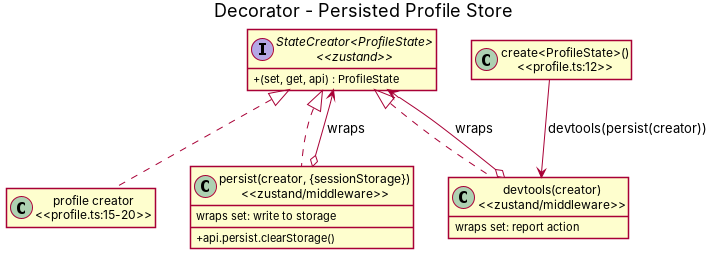
\includegraphics[width=0.62\linewidth]{Part1/diagrams/07_decorator_persisted_profile_store.png}\caption{Persisted Profile Store}\end{figure}
\entry{Verification}{Confirmed; same StateCreator interface in and out; other stores use the undecorated creator. Reviewer: \todo{roll no./name}}
\subsubsection*{NextAuth Prisma Persistence Adapter}
\entry{Pattern type and category}{Adapter --- Structural (GoF)}
\entry{Purpose and origin}{NextAuth persists users, accounts and sessions only through its Adapter interface (createUser, getUserByEmail, linkAccount, ...). Origin: dependency (@next-auth/prisma-adapter@1.0.6) configured by application.}
\textbf{Participant mapping}\par
\begin{tabularx}{\linewidth}{@{}p{3.4cm}X>{\raggedright\arraybackslash}p{6.0cm}@{}}\toprule Pattern role & Actual class, interface and function & File and line range\\\midrule
Target & Adapter (next-auth adapter interface) & dependency next-auth@4.22.1 adapters.d.ts:57\\
Adapter & PrismaAdapter(p) & dependency @next-auth/prisma-adapter@1.0.6 dist/index.js:206-264\\
Adaptee & prisma (PrismaClient) & \path{code/src/server/db.ts:9-14}\\
Client & authOptions.adapter used by NextAuth handler & \path{code/src/server/auth.ts:38-64}; \path{code/src/pages/api/auth/[...nextauth].ts:4}\\
\bottomrule\end{tabularx}
\entry{Evidence}{NextAuth persists users, accounts and sessions only through its Adapter interface (createUser, getUserByEmail, linkAccount, ...). PrismaAdapter returns an object implementing those methods by translating them to Prisma calls, e.g. createUser: (data) =\textgreater{} p.user.create(\{data\}) and getUserByEmail: (email) =\textgreater{} p.user.findUnique(\{where:\{email\}\}) (index.js:208-210). The app wires it with adapter: PrismaAdapter(prisma).}
\entry{Diagram}{\path{Part1/diagrams/08_adapter_nextauth_prisma.puml} (editable), \path{Part1/diagrams/08_adapter_nextauth_prisma.png}}
\begin{figure}[H]\centering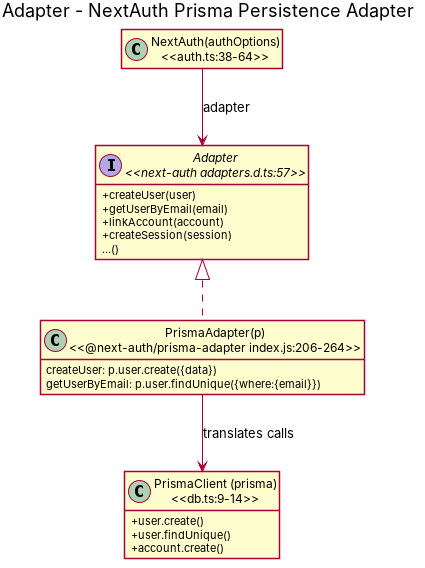
\includegraphics[width=0.62\linewidth]{Part1/diagrams/08_adapter_nextauth_prisma.png}\caption{NextAuth Prisma Persistence Adapter}\end{figure}
\entry{Verification}{Confirmed by reading the adapter source in node\_modules (createUser -> p.user.create, getUserByEmail -> p.user.findUnique). Reviewer: \todo{roll no./name}}
\subsubsection*{Sign-in Provider Strategy}
\entry{Pattern type and category}{Strategy --- Behavioral (GoF)}
\entry{Purpose and origin}{authOptions.providers is a list of interchangeable provider objects behind one Provider type; NextAuth selects the provider by id at sign-in and delegates the authorization/profile mapping to it. Origin: framework (next-auth@4.22.1) configured by application.}
\textbf{Participant mapping}\par
\begin{tabularx}{\linewidth}{@{}p{3.4cm}X>{\raggedright\arraybackslash}p{6.0cm}@{}}\toprule Pattern role & Actual class, interface and function & File and line range\\\midrule
Strategy & Provider = OAuthConfig \textbar{} EmailConfig \textbar{} CredentialsConfig & dependency next-auth@4.22.1 providers/index.d.ts:14\\
ConcreteStrategy & GoogleProvider(\{clientId, clientSecret\}) & \path{code/src/server/auth.ts:50-53}\\
Context & NextAuth(authOptions) with providers[] & \path{code/src/server/auth.ts:38-64}; \path{code/src/pages/api/auth/[...nextauth].ts:4}\\
\bottomrule\end{tabularx}
\entry{Evidence}{authOptions.providers is a list of interchangeable provider objects behind one Provider type; NextAuth selects the provider by id at sign-in and delegates the authorization/profile mapping to it. Only Google is configured; the commented block at auth.ts:54-62 documents adding more without changing NextAuth. Single concrete strategy, so variability is latent.}
\entry{Diagram}{\path{Part1/diagrams/09_strategy_signin_provider.puml} (editable), \path{Part1/diagrams/09_strategy_signin_provider.png}}
\entry{Verification}{Confirmed with the caveat of a single configured strategy (latent variability). Reviewer: \todo{roll no./name}}
\subsubsection*{TMDB Catalogue Facade}
\entry{Pattern type and category}{Facade --- Structural (GoF)}
\entry{Purpose and origin}{Pages need categorised show lists, not URLs. Origin: application.}
\textbf{Participant mapping}\par
\begin{tabularx}{\linewidth}{@{}p{3.4cm}X>{\raggedright\arraybackslash}p{6.0cm}@{}}\toprule Pattern role & Actual class, interface and function & File and line range\\\midrule
Facade & module lib/fetchers: getShows, getNewAndPopularShows, searchShows & \path{code/src/lib/fetchers.ts:5-77,82-122,124-142}\\
Subsystem & TMDB REST endpoints (trending, top\_rated, discover, popular, search/multi) + API key & \path{code/src/lib/fetchers.ts:15-41}; \path{code/src/env.mjs}\\
Client & Home, MoviesPage, TVShowsPage & \path{code/src/app/(shows)/page.tsx:8-52}; \path{code/src/app/(shows)/movies/page.tsx:13-54}; \path{code/src/app/(shows)/tv-shows/page.tsx:12-51}\\
Client & NewAndPopularPage & \path{code/src/app/(shows)/new-and-popular/page.tsx:12-39}\\
Client & SiteHeader.searchShowsByQuery & \path{code/src/components/layouts/site-header.tsx:51-55}\\
\bottomrule\end{tabularx}
\entry{Evidence}{Pages need categorised show lists, not URLs. getShows(mediaType) issues eight TMDB requests in parallel, checks all responses, parses JSON and returns one object of named rows; callers only call getShows('movie'). URL construction, API key, network errors and JSON shape are hidden behind three functions (module-level facade, no class).}
\entry{Diagram}{\path{Part1/diagrams/10_facade_tmdb_catalogue.puml} (editable), \path{Part1/diagrams/10_facade_tmdb_catalogue.png}}
\begin{figure}[H]\centering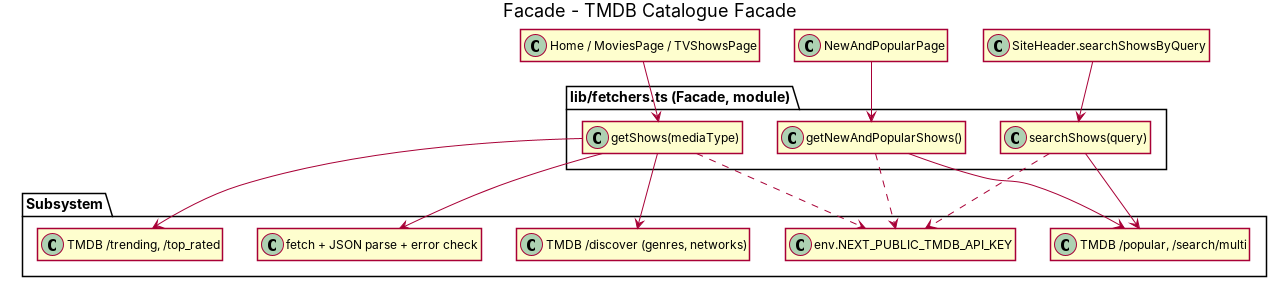
\includegraphics[width=\linewidth]{Part1/diagrams/10_facade_tmdb_catalogue.png}\caption{TMDB Catalogue Facade}\end{figure}
\entry{Verification}{Confirmed; facade behaviour pinned by characterization tests (URLs, order, keys, errors). Reviewer: \todo{roll no./name}}
\subsubsection*{API Router Tree}
\entry{Pattern type and category}{Composite --- Structural (GoF); tRPC router tree}
\entry{Purpose and origin}{createTRPCRouter accepts a record whose values are procedures (leaves) or routers (composites); appRouter nests four routers that hold 19 procedures. Origin: application on framework (@trpc/server).}
\textbf{Participant mapping}\par
\begin{tabularx}{\linewidth}{@{}p{3.4cm}X>{\raggedright\arraybackslash}p{6.0cm}@{}}\toprule Pattern role & Actual class, interface and function & File and line range\\\midrule
Component & AnyRouter \textbar{} AnyProcedure in ProcedureRouterRecord & dependency @trpc/server@10.28.0\\
Composite (root) & appRouter & \path{code/src/server/api/root.ts:12-17}\\
Composite & userRouter & \path{code/src/server/api/routers/user.ts:9-91}\\
Composite & profileRouter & \path{code/src/server/api/routers/profile.ts:6-186}\\
Composite & iconRouter & \path{code/src/server/api/routers/icon.ts:5-59}\\
Composite & myListRouter & \path{code/src/server/api/routers/my-list.ts:6-184}\\
Leaf & 19 procedures e.g. profile.getAll & \path{code/src/server/api/routers/profile.ts:7-15}\\
Factory & createTRPCRouter = t.router & \path{code/src/server/api/trpc.ts:97}\\
\bottomrule\end{tabularx}
\entry{Evidence}{createTRPCRouter accepts a record whose values are procedures (leaves) or routers (composites); appRouter nests four routers that hold 19 procedures. Clients address any node uniformly by dotted path (api.profile.getAll), and the type AppRouter is the whole tree. The recursive DecoratedProcedureRecord type (src/@trpc/next-layout/server/createTrpcNextLayout.tsx:53-65) walks routers and procedures the same way.}
\entry{Diagram}{\path{Part1/diagrams/11_composite_api_router_tree.puml} (editable), \path{Part1/diagrams/11_composite_api_router_tree.png}}
\entry{Verification}{Confirmed; uniform dotted-path access to routers and procedures; 19 leaves. Reviewer: \todo{roll no./name}}
\subsubsection*{Pages-Router tRPC Client Proxy}
\entry{Pattern type and category}{Proxy --- Structural (GoF); remote proxy}
\entry{Purpose and origin}{Components call api.myList.getAll.useQuery(...) as if the server router were local. Origin: application on dependency (@trpc/next@10.28.0).}
\textbf{Participant mapping}\par
\begin{tabularx}{\linewidth}{@{}p{3.4cm}X>{\raggedright\arraybackslash}p{6.0cm}@{}}\toprule Pattern role & Actual class, interface and function & File and line range\\\midrule
Subject & AppRouter type & \path{code/src/server/api/root.ts:20}\\
RealSubject & appRouter served by createNextApiHandler & \path{code/src/pages/api/trpc/[trpc].ts:8-19}\\
Proxy & api = createTRPCNext\textless{}AppRouter\textgreater{}(...) & \path{code/src/lib/api/api.ts:21-54}\\
Transport & loggerLink + httpBatchLink(/api/trpc) & \path{code/src/lib/api/api.ts:36-45}\\
Client & ShowsContainer, ShowModal, ProfilesScreen, SiteHeader and 7 more components & \path{code/src/components/shows-container.tsx:32-36}; \path{code/src/components/show-modal.tsx:93-124}\\
\bottomrule\end{tabularx}
\entry{Evidence}{Components call api.myList.getAll.useQuery(...) as if the server router were local. api is a JavaScript Proxy (createRecursiveProxy/createFlatProxy, @trpc/server dist index-4a823936.js:55,87) that turns each property path into an HTTP batch request to /api/trpc and returns typed results. Same typed interface as the real router (AppRouter).}
\entry{Diagram}{\path{Part1/diagrams/12_proxy_pages_router_trpc_client.puml} (editable), \path{Part1/diagrams/12_proxy_pages_router_trpc_client.png}}
\entry{Verification}{Confirmed; JS Proxy objects in @trpc/server dist (index-4a823936.js:55,87). Reviewer: \todo{roll no./name}}
\subsubsection*{App-Router tRPC Client Proxy}
\entry{Pattern type and category}{Proxy --- Structural (GoF); remote proxy}
\entry{Purpose and origin}{A second client proxy built with the vendored createTRPCNextBeta returns createFlatProxy((key) =\textgreater{} ...) (createTrpcNextBeta.tsx:76-92): 'Provider' and 'useContext' are served locally, every other key is decorated into React-Query hooks that call the server. Origin: application (vendored src/@trpc/next-layout) on dependency.}
\textbf{Participant mapping}\par
\begin{tabularx}{\linewidth}{@{}p{3.4cm}X>{\raggedright\arraybackslash}p{6.0cm}@{}}\toprule Pattern role & Actual class, interface and function & File and line range\\\midrule
Subject & AppRouter type & \path{code/src/server/api/root.ts:20}\\
RealSubject & appRouter served by createNextApiHandler & \path{code/src/pages/api/trpc/[trpc].ts:8-19}\\
Proxy & api = createTRPCNextBeta\textless{}AppRouter\textgreater{}(...) & \path{code/src/lib/api/client.ts:22-45}\\
Proxy factory & createTRPCNextBeta -\textgreater{} createFlatProxy & \path{code/src/@trpc/next-layout/client/createTrpcNextBeta.tsx:48-93}\\
Provider & TRPCProvider wraps RootLayout & \path{code/src/context/trpc-provider.tsx:7-9}; \path{code/src/app/layout.tsx:80-96}\\
Client & AddProfileForm, EditProfileForm & \path{code/src/components/forms/add-profile-form.tsx:13}; \path{code/src/components/forms/edit-profile-form.tsx:15}\\
\bottomrule\end{tabularx}
\entry{Evidence}{A second client proxy built with the vendored createTRPCNextBeta returns createFlatProxy((key) =\textgreater{} ...) (createTrpcNextBeta.tsx:76-92): 'Provider' and 'useContext' are served locally, every other key is decorated into React-Query hooks that call the server. It also supplies the QueryClient used by the app. Two independent proxies for one Subject is recorded as a smell (duplicated getBaseUrl/links).}
\entry{Diagram}{\path{Part1/diagrams/13_proxy_app_router_trpc_client.puml} (editable), \path{Part1/diagrams/13_proxy_app_router_trpc_client.png}}
\entry{Verification}{Confirmed; separate instance because it is a different proxy object built by vendored code; the duplication of two clients is noted as a smell. Reviewer: \todo{roll no./name}}
\subsubsection*{Environment Secret Guard}
\entry{Pattern type and category}{Proxy --- Structural (GoF); protection proxy}
\entry{Purpose and origin}{Server secrets (STRIPE\_API\_KEY, DATABASE\_URL, ...) must never be read in browser bundles. Origin: application (create-t3-app scaffold).}
\textbf{Participant mapping}\par
\begin{tabularx}{\linewidth}{@{}p{3.4cm}X>{\raggedright\arraybackslash}p{6.0cm}@{}}\toprule Pattern role & Actual class, interface and function & File and line range\\\midrule
Subject & MergedOutput (validated env shape) & \path{code/src/env.mjs:67-71}\\
RealSubject & parsed.data (zod-validated variables) & \path{code/src/env.mjs:75-90}\\
Proxy & env = new Proxy(parsed.data, \{get\}) & \path{code/src/env.mjs:92-105}\\
Client & 10 modules importing env, e.g. lib/stripe.ts, lib/fetchers.ts, server/db.ts & \path{code/src/lib/stripe.ts:1-7}; \path{code/src/server/db.ts:3}\\
\bottomrule\end{tabularx}
\entry{Evidence}{Server secrets (STRIPE\_API\_KEY, DATABASE\_URL, ...) must never be read in browser bundles. Every module imports `env`, which is a Proxy whose get trap checks the caller side: on the client any non NEXT\_PUBLIC\_ key throws a descriptive error, otherwise the value is forwarded from the validated object (env.mjs:93-103). Same interface as the real object, access control added transparently.}
\entry{Diagram}{\path{Part1/diagrams/15_proxy_environment_secret_guard.puml} (editable), \path{Part1/diagrams/15_proxy_environment_secret_guard.png}}
\begin{figure}[H]\centering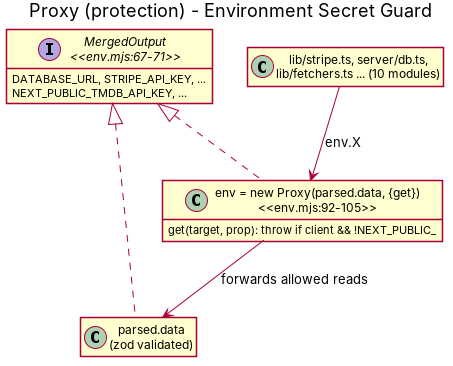
\includegraphics[width=0.62\linewidth]{Part1/diagrams/15_proxy_environment_secret_guard.png}\caption{Environment Secret Guard}\end{figure}
\entry{Verification}{Confirmed (found in the second pass); same mechanism reproduced in Part 3 problem 09. Reviewer: \todo{roll no./name}}
\subsubsection*{My List Query Cache}
\entry{Pattern type and category}{Read-Through Cache --- Architecture (caching); React Query}
\entry{Purpose and origin}{useQuery(key) returns cached data for the key (profile id) and only calls the loader on a miss or after invalidation; with staleTime Infinity, repeated renders of ShowsContainer and ShowModal share one fetch. Origin: application configuration on dependency (@tanstack/react-query@4.29.7).}
\textbf{Participant mapping}\par
\begin{tabularx}{\linewidth}{@{}p{3.4cm}X>{\raggedright\arraybackslash}p{6.0cm}@{}}\toprule Pattern role & Actual class, interface and function & File and line range\\\midrule
Cache & QueryClient created once per TRPCProvider & \path{code/src/@trpc/next-layout/client/createTrpcNextBeta.tsx:55-63}\\
Cache policy & cacheTime: Infinity, staleTime: Infinity, refetchOnWindowFocus: false & \path{code/src/lib/api/client.ts:24-34}\\
Loader (data source) & myListRouter.getAll & \path{code/src/server/api/routers/my-list.ts:7-12}\\
Reader & ShowsContainer myShowsQuery & \path{code/src/components/shows-container.tsx:32-36}\\
Reader & ShowModal myShowsQuery & \path{code/src/components/show-modal.tsx:98-102}\\
Invalidator & ShowModal effect apiUtils.myList.getAll.invalidate() & \path{code/src/components/show-modal.tsx:127-130}\\
\bottomrule\end{tabularx}
\entry{Evidence}{useQuery(key) returns cached data for the key (profile id) and only calls the loader on a miss or after invalidation; with staleTime Infinity, repeated renders of ShowsContainer and ShowModal share one fetch. After each add/remove mutation ShowModal invalidates the key so the next read reloads. Caller never talks to the data source directly.}
\entry{Diagram}{\path{Part1/diagrams/14_cache_my_list_query_cache.puml} (editable), \path{Part1/diagrams/14_cache_my_list_query_cache.png}}
\entry{Verification}{Confirmed; cache behaviour reproduced in Part 3 problem 10. Uncertainty: two client proxies share one React-Query context; not observed at run time here. Reviewer: \todo{roll no./name}}
\subsection*{Rejected and uncertain candidates}
\begin{longtable}{@{}p{4.2cm}p{1.6cm}p{9.8cm}@{}}\toprule Candidate & Decision & Reason\\\midrule\endhead
Caching Proxy for server components (\texttt{createTRPCNextLayout}) & rejected & Proxy + QueryClient structure exists (\path{src/@trpc/next-layout/server/createTrpcNextLayout.tsx:89-168}) but nothing imports it: dead code.\\
Factory Method (\texttt{createTRPCContext}) & rejected & Plain factory functions, no creator hierarchy or overridable creation step.\\
Repository & rejected & Routers call \texttt{ctx.prisma.<model>} directly; no repository abstraction.\\
Template Method (nested layouts) & rejected & Layouts compose children; no base algorithm with overridable steps.\\
Recommendation strategy/engine & rejected & Fixed TMDB queries only (\path{app/(shows)/page.tsx:13-42}); no recommendation logic exists.\\
Debounce & rejected & UI timing technique (\path{components/debounced-input.tsx:44-50}), not a design pattern.\\
Observer via Stripe webhook & uncertain & Only the subscriber side is in code; registration lives in the Stripe dashboard; dispatch is an if-chain on \texttt{event.type}.\\
Protection Proxy for the PIN gate & uncertain & \texttt{ProfilesScreen} conditionally renders children; no common interface. The PIN is sent to the browser and compared there (\path{forms/pin-form.tsx:19}), so it is not real access control.\\
Implicit Next.js data cache & uncertain & \texttt{fetch} in server components is cached by Next 13 by default, but the code sets no option and it was not observed at run time.\\
Facade over session/subscription helpers & uncertain & \path{lib/session.ts:4-11}, \path{lib/subscription.ts:6-53} are thin single-subsystem wrappers.\\\bottomrule
\end{longtable}

\section{Part 2 Evolution and refactoring}
All three changes were implemented on branch \texttt{a12-evolution}. Before any change, commit \texttt{d68c773} added vitest and \emph{characterization tests} that pin the baseline behaviour (no production code changed; 13/13 pass). Characterization tests added later for refactored code were first run on the untouched baseline (19/19, \path{Part2/evidence/tests_baseline_characterization.log}). The four requirements of the case study are covered: \emph{premium content} and the \emph{new subscription plan} in CH01, \emph{regional restrictions} in CH02, \emph{parental control} in CH03. Patches: \path{Part2/changes/patches/0001..0004}; evolved source: \path{Part2/code/}.
\subsection*{CH01 --- Premium content and a new subscription plan (Ultra)}
\entry{Change and acceptance criteria}{New plan \textbf{Ultra} (tier 5, 12.99/month, 4K+HDR, up to \textbf{7 profiles}). Titles of the originals row (TMDB network 213) are \textbf{premium} and playable only with Standard, Premium or Ultra (tier $\ge 3$); other viewers see the title with an ``Upgrade to watch'' button. Acceptance (all automated in \path{tests/ch01-premium-plan.test.ts}): five plans incl.\ Ultra; UI and server plan lists identical; premium title denied for tiers 0--2 and allowed for 3--5; Basic subscriber denied, Standard allowed, anonymous \texttt{UNAUTHORIZED}; Ultra may create a 6th/7th profile but not an 8th, Standard keeps 5; only the originals row tagged premium; all earlier tests pass.}
\entry{Before and after}{commits \texttt{d68c773} $\rightarrow$ \texttt{3f79642} (22 files, +642/-186 incl.\ tests); diff \path{Part2/changes/Change1/change.diff}, file list \path{Part2/changes/Change1/diffstat.txt}, requirement record \path{Part2/changes/Change1/README.md}.}
\entry{Implementation and tests}{New \path{config/plan-catalog.ts}; \path{config/plans.ts} and \path{config/subscriptions.ts} derived from it; \path{lib/access/*} (\texttt{AccessRule}, \texttt{PremiumContentRule}); \path{server/api/trpc.ts} (\texttt{attachSubscription}, \texttt{subscribedProcedure}); new \path{routers/catalogue.ts}; \path{routers/profile.ts} limit from \texttt{ctx.maxProfiles}; \path{lib/fetchers.ts} tags premium; \path{components/show-modal.tsx} upgrade button; checkout refuses a plan without Stripe price; env \texttt{STRIPE\_ULTRA\_PRICE\_ID}. Test fixture change disclosed: fake \texttt{user.findFirst} returns a plan-less user (a signed-in user always has a row); no assertion changed. Run: \texttt{yarn test} and \texttt{yarn typecheck} in \path{Part2/code}. \textbf{Actual result: 29/29 tests passed, typecheck pass} (\path{Part2/changes/Change1/test_result.log}).}
\entry{Pattern effects}{Authenticated Procedure Pipeline \textbf{extended} (new handler \texttt{attachSubscription}); API Router Tree \textbf{extended} (\texttt{catalogueRouter}); TMDB Catalogue Facade \textbf{modified} (premium tagging); \textbf{newly introduced}: Content Access Rule Chain (CoR) and Access Rule Evaluation Template (Template Method: \texttt{AccessRule.check} fixed, \texttt{evaluate} abstract); all others preserved.}
\entry{Refactoring}{\emph{Shotgun Surgery / duplicated data}: plans existed in \path{config/plans.ts} (UI) and \path{config/subscriptions.ts} (server) and had already drifted (Basic devices ``Phone, Tablet, Computer'' vs ``\ldots, TV''). Root cause: the server list reads secret price ids through the env Protection Proxy, which throws in the browser. Technique: extract a client-safe plan catalogue and derive both lists; \emph{Replace Magic Number} 5 with \texttt{plan.maxProfiles} (default 5). Behaviour preservation: subscription and profile-limit characterization tests unchanged and passing; a new test makes future drift fail.}
\entry{Before/after metrics}{lizard 1.24.1, scope \path{src/} without tests and CSS, identical for every snapshot (\path{Part2/evidence/run_snapshots.sh}).}
\begin{tabularx}{\linewidth}{@{}Xrr@{}}\toprule Measure & baseline & CH01\\\midrule
src files / NLOC / functions & 110 / 6694 / 280 & 115 / 6829 / 297\\
average CCN & 2.31 & 2.35\\
plan data (plans.ts + subscriptions.ts + plan-catalog.ts): NLOC / max CCN & 139 / 0 & 123 / 3\\
tRPC pipeline (server/api/trpc.ts): NLOC / max CCN & 49 / 3 & 63 / 6\\
tests passed & 0 (13/13 at d68c773) & 29/29\\\bottomrule\end{tabularx}
\par Max CCN of the whole \path{src/} is reported as 23 $\rightarrow$ 25 by lizard; this is a \textbf{parser artefact}: the CCN-25 function is the unchanged ``Add to My List'' \texttt{onClick} handler in \path{show-modal.tsx} (body identical, checked by script), which lizard did not detect as a function in the baseline JSX.
\subsection*{CH02 --- Regional restrictions}
\entry{Change and acceptance criteria}{Titles are licensed per territory (\texttt{allowedRegions} or \texttt{blockedRegions}); region from the \texttt{x-vercel-ip-country} header, else \texttt{cf-ipcountry}, else US. Unlicensed titles must not appear in any row and must be refused on direct access; a region-blocked premium title is hidden, not upsold. Acceptance (\path{tests/ch02-region.test.ts}): region normalisation and header priority; tRPC context reads the header; Fight Club (550) hidden in CN, allowed in US; Game of Thrones (1399) allowed in IN, hidden in DE; blocked premium title gives \texttt{REGION\_BLOCKED}; locked titles stay visible, hidden ones are removed; row titles and order unchanged; \texttt{checkAccess} uses the request region.}
\entry{Before and after}{commits \texttt{3f79642} $\rightarrow$ \texttt{e420dcf} (17 files, +499/-231 incl.\ tests); diff \path{Part2/changes/Change2/change.diff}, file list \path{Part2/changes/Change2/diffstat.txt}, requirement record \path{Part2/changes/Change2/README.md}.}
\entry{Implementation and tests}{\path{config/regions.ts}, \path{lib/region.ts}, \path{lib/server-region.ts}; \texttt{RegionRule} placed first in the chain, \texttt{visibleShows}; region in the tRPC context; \path{lib/catalogue.ts} + the four \path{(shows)} pages filter rows on the server. Run: \texttt{yarn test} and \texttt{yarn typecheck} in \path{Part2/code}. \textbf{Actual result: 45/45 tests passed, typecheck pass} (\path{Part2/changes/Change2/test_result.log}).}
\entry{Pattern effects}{Content Access Rule Chain \textbf{extended} (RegionRule linked at the front); Access Rule Evaluation Template \textbf{extended}; TMDB Catalogue Facade \textbf{modified} (internal refactoring, interface preserved); others preserved.}
\entry{Refactoring}{(1) \emph{Duplicate Code / Long Method} in \path{lib/fetchers.ts}: 8 + 4 copies of fetch / ok-check / json / return field and an 8-term \texttt{||} condition. Technique: rows as data + one \texttt{fetchRows} helper (Extract Function). (2) \emph{Duplicate Code}: the same 7-entry title/row array in the Home, Movies and TV pages. Technique: \texttt{GENRE\_ROWS} + \texttt{toCategories} (Extract Function). Behaviour preservation: the URL/order/key/error characterization tests pass on the original and on CH02; row titles pinned (the TV page keeps ``Scary Movies'').}
\entry{Before/after metrics}{lizard 1.24.1, scope \path{src/} without tests and CSS, identical for every snapshot (\path{Part2/evidence/run_snapshots.sh}).}
\begin{tabularx}{\linewidth}{@{}Xrr@{}}\toprule Measure & CH01 & CH02\\\midrule
src files / NLOC / functions & 115 / 6829 / 297 & 119 / 6845 / 322\\
average CCN & 2.35 & 2.25\\
TMDB facade (lib/fetchers.ts): NLOC / max CCN & 126 / 9 & 120 / 3\\
row pages (4 shows pages + lib/catalogue.ts): NLOC / max CCN & 174 / 3 & 116 / 3\\
tests passed & 29 & 45/45\\\bottomrule\end{tabularx}
\subsection*{CH03 --- Parental control}
\entry{Change and acceptance criteria}{Each profile has a maturity rating \textbf{KIDS / TEEN / ADULT} (default ADULT, so existing profiles are unchanged), set on Edit Profile. KIDS hides adult titles and Horror, Thriller, Crime, War; TEEN hides adult titles and Horror. Restricted titles disappear from rows, hero, search and My List of that profile; the server refuses them in \texttt{catalogue.checkAccess} and \texttt{myList.create}; another account's profile id is refused. Acceptance (\path{tests/ch03-parental.test.ts}): 9 rating cases; chain order region $\rightarrow$ maturity $\rightarrow$ premium; client filter only for restricted profiles; foreign profile \texttt{FORBIDDEN}; Kids profile cannot save horror; rating stored by \texttt{profile.update}.}
\entry{Before and after}{commits \texttt{e420dcf} $\rightarrow$ \texttt{f393031} (19 files, +536/-147 incl.\ tests); diff \path{Part2/changes/Change3/change.diff}, file list \path{Part2/changes/Change3/diffstat.txt}, requirement record \path{Part2/changes/Change3/README.md}.}
\entry{Implementation and tests}{\texttt{enum MATURITY} + \texttt{Profile.maturityLevel} in \path{prisma/schema.prisma} (apply with \texttt{prisma db push}); \path{config/maturity.ts}; \texttt{MaturityRule} between Region and Premium; \texttt{profileVisibleShows}; \texttt{catalogue.checkAccess} loads the profile with an owner check; maturity guard in \texttt{myList.create}; rating selector in \path{edit-profile-form.tsx}; filtering in \texttt{ShowsContainer}, \texttt{Hero}, search grid. Run: \texttt{yarn test} and \texttt{yarn typecheck} in \path{Part2/code}. \textbf{Actual result: 65/65 tests passed, typecheck pass} (\path{Part2/changes/Change3/test_result.log}).}
\entry{Pattern effects}{Content Access Rule Chain and Access Rule Evaluation Template \textbf{extended} (MaturityRule); Active Profile Selection \textbf{extended} (Hero becomes a new observer, selector on \texttt{maturityLevel}); Search Results Broadcast \textbf{modified} (ShowsContainer filters the broadcast results); Persisted Profile Store preserved (persisted profile now carries the rating); others preserved.}
\entry{Refactoring}{\emph{Duplicate Code} in \path{routers/my-list.ts}: identical 17-field zod schema twice, the ``load profile or NOT\_FOUND'' block three times, field-by-field copies twice. Technique: Extract Variable (\texttt{showInput}), Extract Function (\texttt{findProfileWithList}, \texttt{findShowOrThrow}, \texttt{showData}). Behaviour preservation: \path{tests/characterization-mylist.test.ts} (update/delete errors and written data) ran on the original first and passes on CH03.}
\entry{Before/after metrics}{lizard 1.24.1, scope \path{src/} without tests and CSS, identical for every snapshot (\path{Part2/evidence/run_snapshots.sh}).}
\begin{tabularx}{\linewidth}{@{}Xrr@{}}\toprule Measure & CH02 & CH03\\\midrule
src files / NLOC / functions & 119 / 6845 / 322 & 120 / 6916 / 328\\
average CCN & 2.25 & 2.26\\
my-list router (routers/my-list.ts): NLOC / max CCN & 169 / 3 & 114 / 3\\
access chain (lib/access/*): NLOC / max CCN & 116 / 7 & 168 / 7\\
tests passed & 45 & 65/65\\\bottomrule\end{tabularx}
\begin{figure}[H]\centering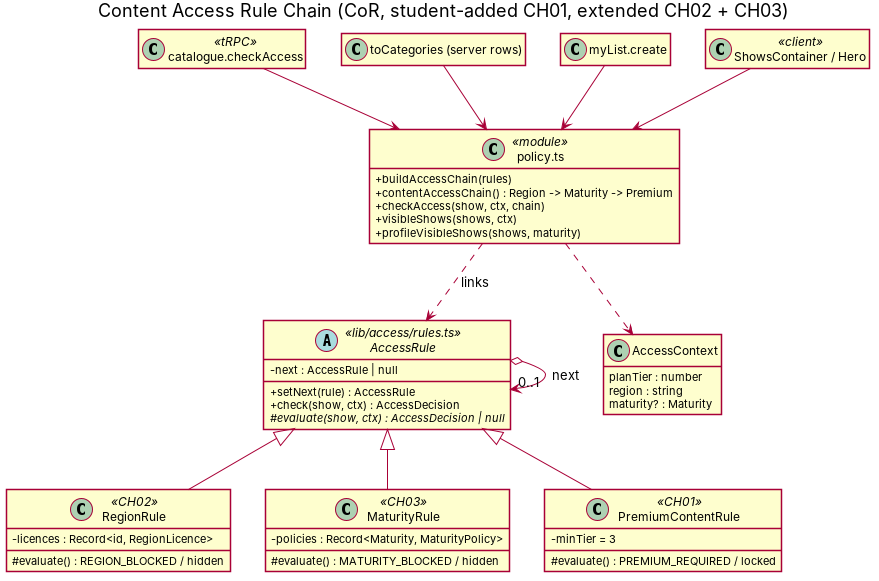
\includegraphics[width=0.85\linewidth]{Part2/diagrams/01_content_access_rule_chain_CH03.png}
\caption{Newly introduced Content Access Rule Chain after CH03 (\texttt{Part2/diagrams/01\_content\_access\_rule\_chain\_CH03.puml}).}\end{figure}
\begin{figure}[H]\centering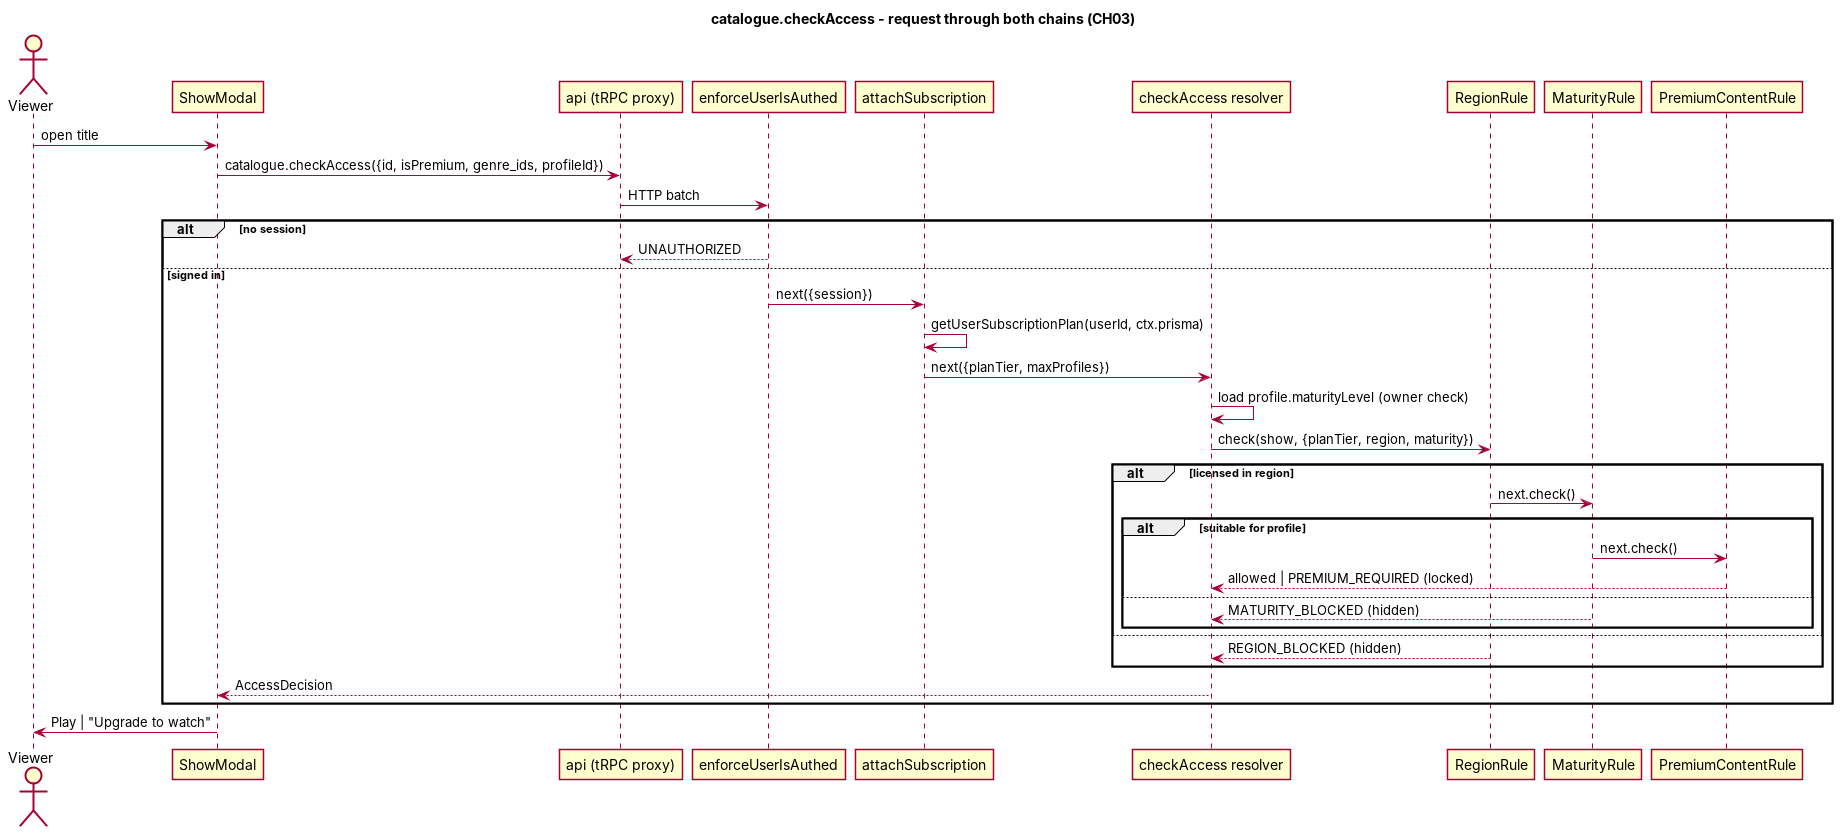
\includegraphics[width=\linewidth]{Part2/diagrams/02_content_access_sequence_CH03.png}
\caption{One \texttt{catalogue.checkAccess} request through both chains (auth middleware chain and access rule chain).}\end{figure}
Further updated UML: \path{Part2/diagrams/03_template_method_access_rule_CH03}, \path{04_cor_authenticated_pipeline_CH01}, \path{05_composite_api_router_tree_CH01}, \path{06_observer_active_profile_selection_CH03}, \path{07_facade_tmdb_refactored_CH02}, \path{08_plan_catalogue_refactor_CH01} (\texttt{.puml} + \texttt{.png}).
\subsection{Updated pattern counts}
Counts per snapshot (\path{data/pattern_counts.csv}); rows with participants, locations, status and change description per instance and snapshot in \path{data/pattern_evolution.csv} (66 rows; all 246 evolved locations re-measured and checked).

\begin{tabularx}{\linewidth}{@{}lXcccc@{}}\toprule Snapshot & Change in counts & Types & Instances & Concrete & Rejected / uncertain\\\midrule
baseline 676e5dd & --- & 10 & 15 & 33 & 6 / 4\\
CH01 3f79642 & + Content Access Rule Chain (CoR), + Access Rule Evaluation Template (new type Template Method) & 11 & 17 & 37 & 6 / 4\\
CH02 e420dcf & instances continue (RegionRule added) & 11 & 17 & 39 & 6 / 4\\
CH03 f393031 & instances continue (MaturityRule, Hero observer) & 11 & 17 & 42 & 6 / 4\\\bottomrule
\end{tabularx}

Per-type instance counts after CH01--CH03: Chain of Responsibility 2, Observer 3, Proxy 3, Singleton 2, Adapter, Composite, Decorator, Facade, Strategy, Read-Through Cache, Template Method 1 each. No instance was replaced or removed. The two new instances are student-added and share participant classes: the \emph{chain} is the object-level collaboration (links via \texttt{setNext}), the \emph{template} is the class-level one (\texttt{check} fixed in the base class, \texttt{evaluate} overridden). The old Authenticated Procedure Pipeline continues under its name and now feeds the plan tier into the new chain.
\entry{Interpretation}{\textbf{Benefits.} Each new rule was one class plus one line in \texttt{contentAccessChain}; the CH02/CH03 diffs did not touch \texttt{PremiumContentRule}. Ordering ``hide before lock'' is explicit and tested. Extending the existing tRPC chain (\texttt{attachSubscription}) gave every resolver the plan once per request. The refactorings removed real duplication: the facade's max CCN fell 9 $\rightarrow$ 3, the row pages 174 $\rightarrow$ 116 NLOC, the My-List router 169 $\rightarrow$ 114 NLOC, and the plan data shrank 139 $\rightarrow$ 123 NLOC while gaining a fifth plan. \textbf{Trade-offs.} Total NLOC grew 6694 $\rightarrow$ 6916 (+3.3\%) and functions 280 $\rightarrow$ 328, mostly new features and small helpers; more LOC here is not worse design and less LOC alone would not prove better design. The rule chain is evaluated in three places (server rows, tRPC, browser) with different context completeness (rows know region only, the browser knows maturity only). \textbf{Remaining limitations.} Sample licence/premium data; hand-written profile \texttt{select} in four pages (another Shotgun Surgery spot); the persisted profile keeps an old rating until re-selected; pre-existing missing ownership checks on profile/My-List procedures; no end-to-end run with real services.}

\section{Part 3 Cross-language comparison}
\entry{Selected instances}{One verified instance per confirmed baseline type (10 problems). Where a type has several instances we chose the one that best shows the pattern in a small problem: Chain of Responsibility --- \emph{Content Access Rule Chain} (CH03 state; richer than the one-handler auth pipeline and also exercises the Template Method introduced in CH01); Singleton --- \emph{Shared Prisma Database Client} (explicit holder, hot-reload behaviour); Observer --- \emph{Active Profile Selection} (most observers, extended in CH03); Proxy --- \emph{Environment Secret Guard} (protection logic shows the language mechanisms best); Decorator --- Persisted Profile Store; Adapter --- NextAuth Prisma Persistence Adapter; Strategy --- Sign-in Provider Strategy; Facade --- TMDB Catalogue Facade (after CH02); Composite --- API Router Tree (after CH01); Read-Through Cache --- My List Query Cache.}
\entry{Common specifications}{For each problem, \path{Part3/<problem>/test-cases/spec.md} gives inputs, outputs, rules and error cases, and \path{test-cases/cases.tsv} is the \emph{single shared fixture} read by all four test runners (9--16 cases each, 107 in total, including error cases such as unknown maturity, invalid NODE\_ENV, unknown decorator, ORM constraint errors, unsupported provider, invalid media type, server-variable access on the client, missing My-List entry). Test doubles that belong to the problem (fake HTTP client in 07) are defined identically in every runner.}
\entry{Implementations}{Folders \texttt{Part3/NN\_<pattern>\_<problem>/\{java,python,javascript,cpp\}/} with production code, a separate test runner and a README with the run command. Runtimes: javac 21.0.12.1 / openjdk version "21.0.12.1" 2026-08-18; Python 3.13.16; Node.js v22.22.0; g++ (Ubuntu 13.3.0-6ubuntu2\textasciitilde{}24.04.1) 13.3.0 -std=c++17 -O2. Commands (working folder = language folder):
\begin{itemize}
\item Java: \texttt{javac -d build *.java}; \texttt{java -cp build Runner ../test-cases/cases.tsv}
\item Python: \texttt{python3 test\_runner.py ../test-cases/cases.tsv}
\item JavaScript: \texttt{node testRunner.js ../test-cases/cases.tsv}
\item C++: \texttt{g++ -std=c++17 -O2 -Wall -o build/test\_runner test\_runner.cpp}; \texttt{./build/test\_runner ../test-cases/cases.tsv}
\end{itemize}
All forty are built, run, timed and measured by \path{Part3/run_all.py}.}
\entry{Actual results}{\textbf{All 40 implementations pass all their cases} (107 cases $\times$ 4 languages = 428 checks); none marked not run. Logs: \path{Part3/evidence/<problem>_<language>.log}.}
\entry{Static and dynamic comparison}{Rules: LOC = lizard NLOC of production files only; max CC = largest lizard cyclomatic complexity of one function; time = median of 5 runs after 1 warm-up, whole process incl.\ runtime start-up and reading the fixture (raw: \path{Part3/evidence/timings.csv}). Full table with notes: \path{data/cross_language.csv}.}
\begin{longtable}{@{}p{4.6cm}rrrrrrrr@{}}\toprule
& \multicolumn{4}{c}{source LOC} & \multicolumn{4}{c}{median ms}\\
Problem & Java & Py & JS & C++ & Java & Py & JS & C++\\\midrule\endhead
Chain of Responsibility (01) & 69 & 68 & 60 & 86 & 81.7 & 40.1 & 34.8 & 1.9\\
Singleton (02) & 28 & 15 & 17 & 28 & 75.1 & 14.1 & 35.7 & 2.2\\
Observer (03) & 44 & 30 & 24 & 50 & 82.9 & 40.7 & 32.9 & 1.8\\
Decorator (04) & 71 & 37 & 34 & 59 & 93.9 & 15.3 & 33.1 & 2.5\\
Adapter (05) & 50 & 37 & 31 & 59 & 85.6 & 14.1 & 31.7 & 1.8\\
Strategy (06) & 55 & 29 & 31 & 63 & 74.8 & 19.8 & 30.0 & 2.3\\
Facade (07) & 49 & 25 & 34 & 62 & 100.1 & 14.4 & 32.4 & 1.8\\
Composite (08) & 68 & 36 & 36 & 70 & 93.0 & 14.5 & 31.8 & 1.8\\
Proxy (09) & 26 & 11 & 16 & 39 & 101.6 & 13.8 & 31.9 & 1.7\\
Read-Through Cache (10) & 37 & 28 & 33 & 42 & 87.8 & 20.2 & 38.7 & 1.7\\
\midrule Total LOC / median of medians & 497 & 316 & 316 & 558 & 86.7 & 14.9 & 32.6 & 1.8\\
Max function CC (all problems) & 5 & 6 & 5 & 6 & & & & \\\bottomrule\end{longtable}
\entry{Comparison}{\textbf{Participant structures.} The same roles appear in every language, but how they are expressed differs. Java and C++ name every role as a type (interfaces / abstract classes, \texttt{final}/\texttt{override}), so the participant mapping is visible in declarations; Python relies on duck typing (ABC only where an abstract step must be enforced, e.g.\ \texttt{AccessRule.evaluate}); JavaScript often needs no class at all: observers are functions in a \texttt{Set}, decorators are functions \texttt{store $\rightarrow$ store} that spread and override, the adapter is a factory returning an object literal --- exactly the style of zustand, next-auth and tRPC in the source. \textbf{Abstraction and inheritance vs.\ composition.} Template Method needs inheritance in all four (abstract \texttt{check}/\texttt{evaluate}); all other problems use composition: decorators wrap, chains link, the facade holds the HTTP client. In C++ ownership is part of the design (\texttt{unique\_ptr} for chain links and decorators, non-owning pointers for observers, \texttt{shared\_ptr} to keep the singleton's identity across reloads). \textbf{Language features.} Proxy is the clearest difference: JavaScript's built-in \texttt{Proxy} traps property access (identical to \path{env.mjs}); Python's \texttt{\_\_getattr\_\_} intercepts attribute reads; Java's \texttt{java.lang.reflect.Proxy} intercepts interface calls at run time via reflection; C++ has no run-time interception, so the proxy is an ordinary class implementing the same interface. Records/dataclasses/structs give value objects; \texttt{Optional}/\texttt{std::optional}/\texttt{None}/\texttt{null} express ``no result'' in the chain and adapter. JavaScript is the only version of the facade that is asynchronous (\texttt{Promise.all}), like the source. \textbf{Static vs.\ dynamic results.} Python and JavaScript need about 37\% less code than Java and about 45\% less than C++ (316 vs.\ 497 vs.\ 558 NLOC in total); complexity per function is low everywhere (max CC 5--6). Measured times are dominated by start-up: native C++ 1.7--2.5\,ms, Python 14--20\,ms, Node.js 30--39\,ms, JVM 75--100\,ms. The two Python problems that import \texttt{dataclasses} (01, 03) start $\approx$25\,ms slower; \texttt{python3 -X importtime -c "import dataclasses"} measured 19.7--26.2\,ms. The timing therefore compares runtimes, not the patterns.}
\entry{Technology discussion}{The case-study stack implements several patterns in its frameworks, so the application inherits them: tRPC middlewares form a Chain of Responsibility in which each middleware calls \texttt{next()} or stops the request [8]; zustand middlewares (\texttt{persist}, \texttt{devtools}) are decorators over a state creator [9]; NextAuth separates providers (strategies) and database adapters [10]; TanStack Query is a read-through cache with explicit invalidation [11]. JavaScript's \texttt{Proxy} [5] is used both by tRPC (remote proxy) and by the T3 \texttt{env} module (protection proxy), while Java offers dynamic proxies only for interfaces [6] and Python offers attribute hooks [7]. This matches the GoF observation that patterns depend on language features [1]: in a language with first-class functions and proxies several GoF patterns shrink to idioms, which is what the JavaScript column and the source code show.}

\section{LLM records and human verification}
\entry{Run and model}{Claude (claude.ai), displayed model \textbf{Claude Opus 5.5}, access tier \todo{Free / Pro}, 2026-10-10; one conversation covering Parts 1--3 (prompts: \path{Part1/llm/Part1_prompt.txt}, \path{Part2/llm/Part2_prompt.txt}, \path{Part3/llm/part3_prompt.txt}). The model worked in a sandbox with a shell: it cloned the application, ran the typechecker, tests, lizard and the Part 3 programs itself, so its numeric results come from real runs. \todo{if the course requires a free tool, repeat the Part 1 prompt with a free model and add a row to data/llm.csv}}
\entry{Inputs and outputs}{Input: \path{code/} (commit 676e5dd) and the three assignment files. Outputs and claim tables: \path{Part1/llm/llm_output_part1.md}, \path{Part2/llm/llm_output_part2.md}, \path{Part3/llm/llm_output_part3.md}; summary in \path{data/llm.csv}. The raw transcript must be exported from claude.ai into the same folders \todo{export transcript}.}
\entry{Claims and evaluation}{Partially correct, corrected before submission. Errors found by checking the model's own work against the source and tools: (1) first inventory had 14 instances --- the Environment Secret Guard proxy was missed and added on a second pass; (2) three line ranges were wrong (two end lines, one offset) --- found by an independent locator and corrected; (3) first Part 2 NLOC run ignored \texttt{.tsx} files (1617 instead of 6694) --- corrected; (4) a reported max-CCN increase was identified as a lizard parsing artefact. One claim was not accepted: the Stripe webhook as Observer (kept as uncertain). Correct claims include the missing licence, dead caching-proxy code, the client-side PIN check and the 18/19 protected procedures. Reviewer: \todo{roll no./name of the team member who re-checked, with date}}
\entry{Generated code}{All Part 2 production code and tests and all Part 3 code were generated by the model. Use and testing: Part 2 --- characterization tests run on the original before refactoring, acceptance tests per change, 65/65 passing plus typecheck on the final snapshot; Part 3 --- 40 implementations, 428/428 shared-fixture checks. The team must review and be able to explain this code \todo{reviewers per part}.}

\section{Findings, contributions and references}
\entry{Findings}{\begin{itemize}
\item netflx-web uses 10 pattern types in 15 collaborations at the baseline; most come from frameworks and libraries (tRPC, zustand, NextAuth, React Query, T3 scaffold) and are configured, not written, by the application. Observer (3) and Proxy (3) are the most frequent; recommendation has no pattern because it has no logic.
\item The access requirements fitted the existing Chain of Responsibility idea: one tRPC middleware was added and a new rule chain absorbed premium, region and parental rules with one class each; the chain order (hide before lock) is a design decision of its own and is tested.
\item The env Protection Proxy explains a code smell: the plan list was duplicated because the server list reads secrets. Moving the client-safe part into one module removed the duplication and an existing inconsistency.
\item Security observations (pre-existing, reported): the profile PIN is checked in the browser; profile and My-List procedures accept any profileId; the server caching proxy is dead code; two tRPC client proxies exist side by side.
\item Limitations: no end-to-end run with real Stripe, TMDB and Google services; sample licence and premium data; lizard's TSX parsing is imperfect; Part 3 times are start-up dominated and machine-specific.
\end{itemize}}
\entry{Contributions}{\todo{one line per student: actual contribution and link to the files/commits they produced or reviewed}\par\medskip
\begin{tabularx}{\linewidth}{@{}lllX@{}}\toprule Roll number & Name & Batch & Contribution\\\midrule
AM.SC.U4CSE23161 & Swaminathan A & CSE B & \todo{}\\
AM.SC.U4CSE23207 & Anna Ouseph & CSE C & \todo{}\\
AM.SC.U4CSE23230 & Leya Paul & CSE C & \todo{}\\
AM.SC.U4CSE23242 & Pooja Sathyan & CSE C & \todo{}\\
AM.SC.U4CSE23069 & Rahul Rajan & CSE A & \todo{}\\\bottomrule\end{tabularx}}
\entry{References}{\begin{enumerate}[label={[\arabic*]}]
\item E. Gamma, R. Helm, R. Johnson, J. Vlissides, \emph{Design Patterns: Elements of Reusable Object-Oriented Software}, Addison-Wesley, 1994.
\item M. Fowler, \emph{Refactoring: Improving the Design of Existing Code}, 2nd ed., Addison-Wesley, 2018.
\item sadmann7, netflx-web, \url{https://github.com/sadmann7/netflx-web} (commit 676e5dd, accessed 2026-10-10).
\item Next.js documentation, \url{https://nextjs.org/docs}; T3 stack (create-t3-app), \url{https://create.t3.gg}.
\item MDN Web Docs, ``Proxy'', \url{https://developer.mozilla.org/en-US/docs/Web/JavaScript/Reference/Global_Objects/Proxy}.
\item Oracle, Java SE 21 API, \texttt{java.lang.reflect.Proxy}, \url{https://docs.oracle.com/en/java/javase/21/docs/api/java.base/java/lang/reflect/Proxy.html}.
\item Python 3 Language Reference, Data model --- customizing attribute access, \url{https://docs.python.org/3/reference/datamodel.html}.
\item tRPC documentation (procedures and middlewares), \url{https://trpc.io/docs}.
\item zustand (incl.\ \texttt{persist} and \texttt{devtools} middleware), \url{https://github.com/pmndrs/zustand}.
\item NextAuth.js documentation (providers, adapters), \url{https://next-auth.js.org}.
\item TanStack Query v4 documentation (caching, invalidation), \url{https://tanstack.com/query/v4}.
\item lizard code complexity analyser, \url{https://github.com/terryyin/lizard}; PlantUML, \url{https://plantuml.com}; vitest, \url{https://vitest.dev}.
\end{enumerate}}

\section{Team folder and datasets (take a screenshots from the GitHub repository--- your team)}
\todo{insert a screenshot of the A12 folder in the GitHub repository after upload}
\begin{verbatim}
A12/
  README.md
  A12_Report.tex
  A12_Report.pdf
  data/   patterns.csv, pattern_counts.csv, pattern_evolution.csv,
          cross_language.csv, llm.csv
  code/   original application source (676e5dd)
  test_result/baseline/   typecheck, build and characterization logs
  Part1/  diagrams/ (.puml + .png), evidence/, llm/
  Part2/  code/ (evolved source), changes/Change1..3 + patches/,
          diagrams/, evidence/, llm/
  Part3/  NN_<pattern>_<problem>/{java,python,javascript,cpp,test-cases}/,
          evidence/, llm/, run_all.py
\end{verbatim}

\end{document}
